\subsection{Пример работы программы}

Рассмотрим в качестве примера работы программы модель управления скоростью электродвигателя постоянного тока. Данная модель была предложена и исследована на управляемость в \cite{baghdad}. Мы сравним полученные в работе~\cite{baghdad} управления без запаздывания с построенными нами.

Итак, модель представляет собой систему:
\begin{equation}\label{eq:example}
\begin{cases}
\frac{d}{dt}i(t)
=
-\frac{R}{L}i(t)
-
\frac{K_b}{L}\omega(t)
+
\frac{1}{L}u(t),\\
\frac{d}{dt}\omega(t)
=
-\frac{K_T}{J}i(t)
-
\frac{B}{J}\omega(t).
\end{cases}
\end{equation}
Здесь $i,[\mbox{А}]$ --- сила тока на соответстующем участке цепи; $\omega,\left[\frac{\mbox{рад}}{\mbox{с}}\right]$ --- угловая скорость вращения; $u,[\mbox{В}]$ --- управляемое нами напряжение на концах цепи. 

\begin{figure}[bh]


\tikzset{every picture/.style={line width=0.75pt}} %set default line width to 0.75pt        
\centering
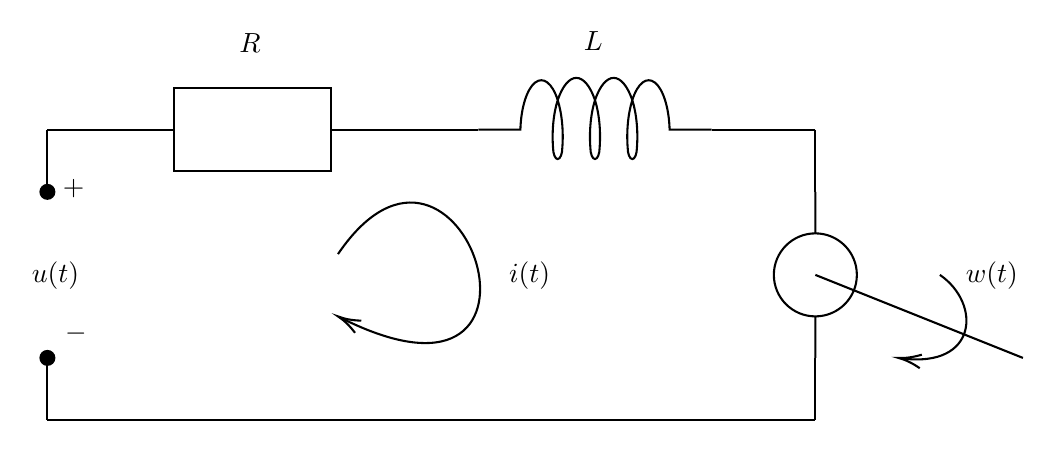
\begin{tikzpicture}[x=0.75pt,y=0.75pt,yscale=-1,xscale=1]
%uncomment if require: \path (0,300); %set diagram left start at 0, and has height of 300

%Shape: Resistor [id:dp759021563450837] 
\draw   (101.18,90) -- (176.49,90) -- (176.49,130) -- (101.18,130) -- (101.18,90) -- cycle (80,110) -- (101.18,110) (176.49,110) -- (197.67,110) ;
%Straight Lines [id:da9833480980865364] 
\draw    (80,110) -- (40,110) ;
%Straight Lines [id:da7530411059484647] 
\draw    (40,110) -- (40,140) ;
\draw [shift={(40,140)}, rotate = 90] [color={rgb, 255:red, 0; green, 0; blue, 0 }  ][fill={rgb, 255:red, 0; green, 0; blue, 0 }  ][line width=0.75]      (0, 0) circle [x radius= 3.35, y radius= 3.35]   ;
%Straight Lines [id:da4394842288276831] 
\draw    (197.67,110) -- (247.67,110) ;
%Shape: Inductor (Air Core) [id:dp1789049029135794] 
\draw   (247.67,110) -- (267.89,110) .. controls (268.18,99.49) and (270.98,90.51) .. (274.96,87.37) .. controls (278.93,84.23) and (283.26,87.57) .. (285.86,95.79) .. controls (287.87,102.2) and (288.69,110.48) .. (288.11,118.53) .. controls (288.11,121.67) and (287.1,124.21) .. (285.86,124.21) .. controls (284.62,124.21) and (283.61,121.67) .. (283.61,118.53) .. controls (283.03,110.48) and (283.85,102.2) .. (285.86,95.79) .. controls (288.19,88.96) and (291.45,85.09) .. (294.85,85.09) .. controls (298.25,85.09) and (301.5,88.96) .. (303.83,95.79) .. controls (305.84,102.2) and (306.66,110.48) .. (306.08,118.53) .. controls (306.08,121.67) and (305.07,124.21) .. (303.83,124.21) .. controls (302.59,124.21) and (301.59,121.67) .. (301.59,118.53) .. controls (301.01,110.48) and (301.83,102.2) .. (303.83,95.79) .. controls (306.17,88.96) and (309.42,85.09) .. (312.82,85.09) .. controls (316.22,85.09) and (319.47,88.96) .. (321.81,95.79) .. controls (323.81,102.2) and (324.63,110.48) .. (324.05,118.53) .. controls (324.05,121.67) and (323.05,124.21) .. (321.81,124.21) .. controls (320.57,124.21) and (319.56,121.67) .. (319.56,118.53) .. controls (318.98,110.48) and (319.8,102.2) .. (321.81,95.79) .. controls (324.41,87.57) and (328.74,84.23) .. (332.71,87.37) .. controls (336.68,90.51) and (339.49,99.49) .. (339.78,110) -- (360,110) ;
%Straight Lines [id:da7540700655846257] 
\draw    (360,110) -- (410,110) ;
%Straight Lines [id:da7535572793540471] 
\draw    (410,110) -- (410,140) ;
%Shape: Output [id:dp058288178798897916] 
\draw   (410,160) .. controls (421.05,160) and (430,168.95) .. (430,180) .. controls (430,191.05) and (421.05,200) .. (410,200) .. controls (398.95,200) and (390,191.05) .. (390,180) .. controls (390,168.95) and (398.95,160) .. (410,160) -- cycle (410,140) -- (410,160) (410,220) -- (410,200) ;
%Straight Lines [id:da6255843491047207] 
\draw    (410,220) -- (410,250) ;
%Straight Lines [id:da6133494645345363] 
\draw    (40,250) -- (410,250) ;
%Straight Lines [id:da9318737388527801] 
\draw    (40,220) -- (40,250) ;
\draw [shift={(40,220)}, rotate = 90] [color={rgb, 255:red, 0; green, 0; blue, 0 }  ][fill={rgb, 255:red, 0; green, 0; blue, 0 }  ][line width=0.75]      (0, 0) circle [x radius= 3.35, y radius= 3.35]   ;
%Curve Lines [id:da4185870543351564] 
\draw    (180,170) .. controls (239.37,82.44) and (297.75,258.89) .. (181.76,200.89) ;
\draw [shift={(180,200)}, rotate = 387.14] [color={rgb, 255:red, 0; green, 0; blue, 0 }  ][line width=0.75]    (10.93,-3.29) .. controls (6.95,-1.4) and (3.31,-0.3) .. (0,0) .. controls (3.31,0.3) and (6.95,1.4) .. (10.93,3.29)   ;
%Straight Lines [id:da13172357267529422] 
\draw    (410,180) -- (510,220) ;
%Curve Lines [id:da7742183141810091] 
\draw    (470,180) .. controls (490.03,193.79) and (488.39,225.04) .. (451.7,220.24) ;
\draw [shift={(450,220)}, rotate = 368.9] [color={rgb, 255:red, 0; green, 0; blue, 0 }  ][line width=0.75]    (10.93,-3.29) .. controls (6.95,-1.4) and (3.31,-0.3) .. (0,0) .. controls (3.31,0.3) and (6.95,1.4) .. (10.93,3.29)   ;

% Text Node
\draw (131,62.4) node [anchor=north west][inner sep=0.75pt]    {$R$};
% Text Node
\draw (297,61.4) node [anchor=north west][inner sep=0.75pt]    {$L$};
% Text Node
\draw (46,132.4) node [anchor=north west][inner sep=0.75pt]    {$+$};
% Text Node
\draw (47,202.4) node [anchor=north west][inner sep=0.75pt]    {$-$};
% Text Node
\draw (31,172.4) node [anchor=north west][inner sep=0.75pt]    {$u( t)$};
% Text Node
\draw (261,172.4) node [anchor=north west][inner sep=0.75pt]    {$i( t)$};
% Text Node
\draw (481,172.4) node [anchor=north west][inner sep=0.75pt]    {$w( t)$};
\end{tikzpicture}
\caption{Схема электрической цепи электродвигателя постоянного тока.}
\end{figure}

Ниже приведем таблицу с описанием констант в системе \eqref{eq:example} и их характерными значениями для электродвигателя постоянного тока:

\begin{center}
\begin{tabular}{|c|l|c|}
\hline
Обозначение
&
Физ. величина
&
Хар. значение\\
\hline
&&\\
$J$
&
Момент инерции
&
$0,\!01\;\frac{\mbox{кг}\cdot\mbox{м}^2}{\mbox{рад}}$\\
\hline
&&\\
$B$
&
Коэффициент вязкого трения
&
$0,\!1\;\frac{\mbox{кг}\cdot\mbox{м}\cdot\mbox{с}}{\mbox{рад}}$
\\
\hline
&&\\
$K_T$
&
Постоянная кручения
&
$0,\!01\;\frac{\mbox{Н}\cdot\mbox{м}}{\mbox{А}}$
\\
\hline
&&\\
$K_b$
&
Постоянная ЭДС
&
$0,\!01\;\frac{\mbox{В}\cdot\mbox{с}}{\mbox{рад}}$
\\
\hline
&&\\
$R$
&
Сопротивление резистора
&
$1\;\mbox{Ом}$
\\
\hline
&&\\
$L$
&
Индуктивность катушки
&
$0,\!5\;\mbox{Гн}$
\\
\hline
\end{tabular}
\end{center}

Таким образом, мы приходим к удобному нам виду уравнения:
\begin{equation}\label{eq:x-example}
        \frac{dx}{dt}
        =
        \begin{pmatrix}
-2 & -0,\!02 \\
-1 & -10
        \end{pmatrix}
        x
        +
        \begin{pmatrix}
2 \\
0
        \end{pmatrix}
        u.
\end{equation}
Для него мы поставим задачу минимизации на отрезке $1 \leqslant t \leqslant 3$ функционала \eqref{eq:functional} с матрицами:
$$
        M = \begin{pmatrix}
1 & 0 \\
0 & 10
        \end{pmatrix},
        \quad
        N = (1),
        \quad
        T = \begin{pmatrix}
1 & 0 \\
0 & 1
        \end{pmatrix}.
$$
Начальными условиями будут:
$$
        x(1) = \begin{pmatrix}
4 \\
100
        \end{pmatrix}.
$$
\begin{figure}[bh]
        \noindent\centering{
        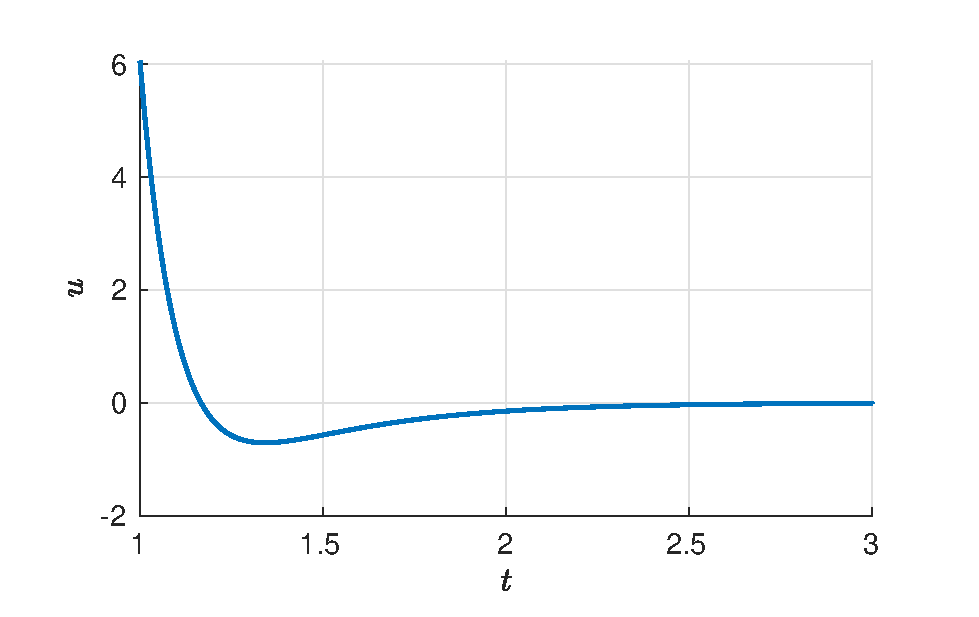
\includegraphics[width=160mm]{content/continuous_task/example/simple-control.eps}
        }
        \caption{Оптимальная стратегия без запаздывания наблюдения для системы~\eqref{eq:x-example}. Значение функционала $J = 4970,\!8$.}
        \label{img:simple-control}
\end{figure}
\begin{figure}[bh]
        \noindent\centering{
        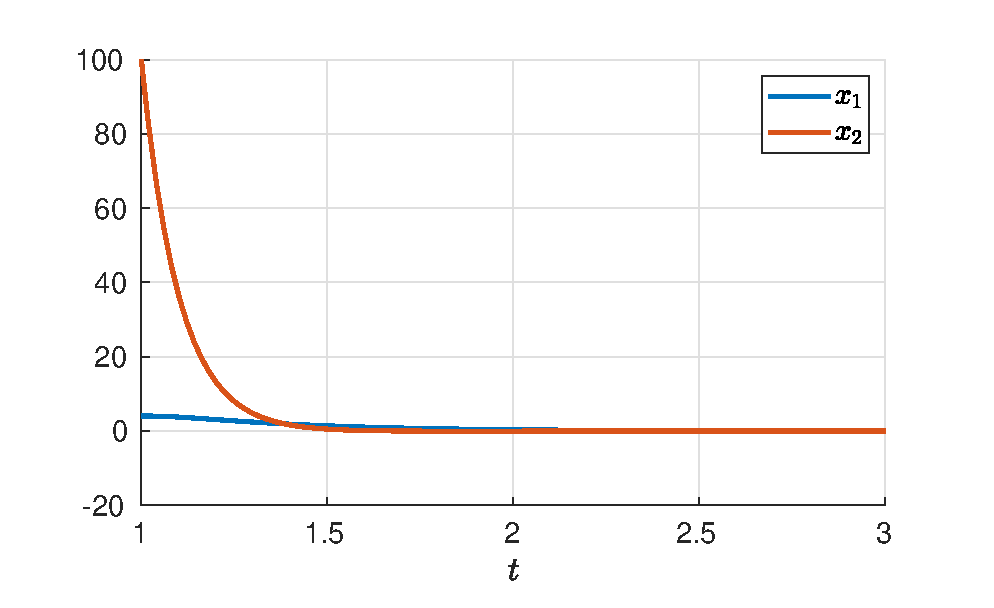
\includegraphics[width=160mm]{content/continuous_task/example/simple-tr.eps}
        }
        \caption{Поведение системы \eqref{eq:x-example} при использовании оптимальной стратегии без запаздывания наблюдения.}
        \label{img:simple-tr}
\end{figure}

На рисунках Рис.~\ref{img:simple-control} и Рис.~\ref{img:simple-tr} можно посмотреть оптимальное управление и поведение системы \eqref{eq:x-example} для задачи без запаздывания по наблюдению. С этими графиками мы будем сравнивать управления, построенные по нашему алгоритму. Значение функционала при такой постановке задачи равно $J = 4970,8$.

Теперь построем управление по нашему алгоритму. Будем считать, что запаздывание по наблюдению равно $h = 0,\!5$. Возьмем мелкое разбиение $\varepsilon = 10^{-2}$. Как видно из рисунков Рис.~\ref{img:small-control} и Рис.~\ref{img:small-tr} построенное управление практически не отличается от случая без запаздывания, что соответствует приведённой теории. Значение функционала $J = 4971$.

Предложенный алгоритм предполагает вычисление $\left\lceil\frac{h}{\varepsilon}\right\rceil$ интегралов на каждом шаге работы программы. Это значит, что при увеличении времени задержки, время работы программы так же будет увеличиваться. Если на каждом шаге программы запоминать вычисленное положение $x(t - \varepsilon)$, то можно сократить количество интегралов до одного. График сравнения времени работы программы с и без улучшения алгоритма предствавлен на рисунке Рис.~\ref{img:cpu}.

\begin{figure}[bh]
        \noindent\centering{
        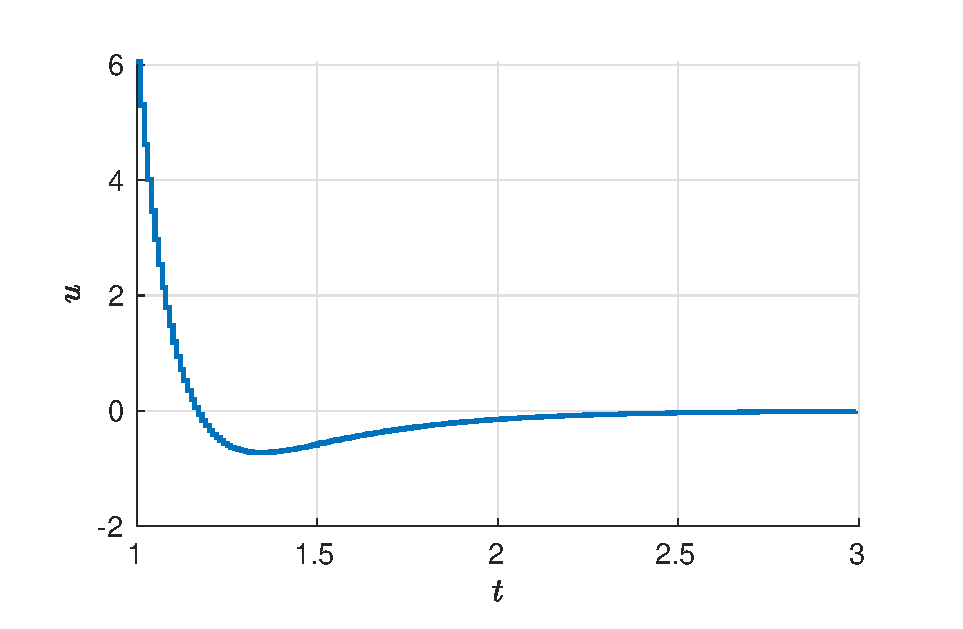
\includegraphics[width=160mm]{content/continuous_task/example/small-control.eps}
        }
        \caption{Оптимальная стратегия с запаздыванием наблюдения $h = 0,\!5$ для системы~\eqref{eq:x-example} с разбиением $\varepsilon = 0,\!01$. Значение функционала $J = 4971$.}
        \label{img:small-control}
\end{figure}
\begin{figure}[bh]
        \noindent\centering{
        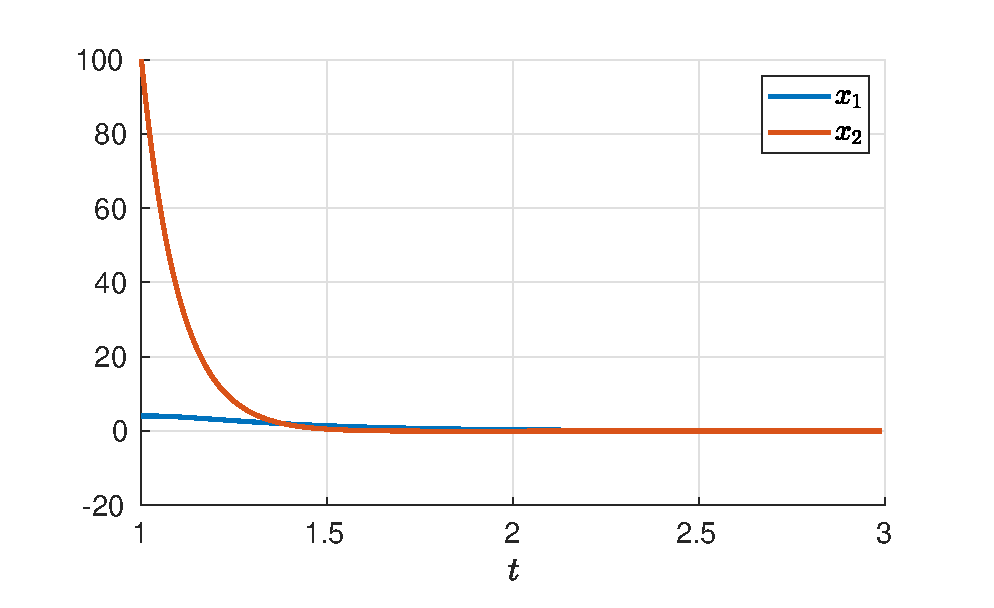
\includegraphics[width=160mm]{content/continuous_task/example/small-tr.eps}
        }
        \caption{Поведение системы \eqref{eq:x-example} при использовании оптимальной стратегии c запаздыванием наблюдения (Рис.~\ref{img:small-control}).}
        \label{img:small-tr}
\end{figure}
\begin{figure}[bh]
        \noindent\centering{
        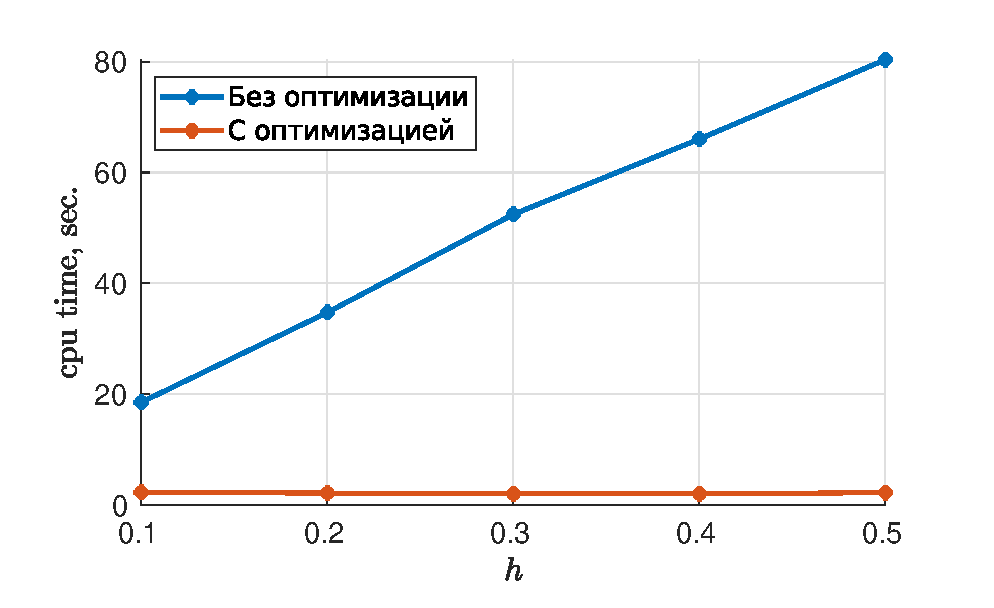
\includegraphics[width=160mm]{content/continuous_task/example/cpu.eps}
        }
        \caption{Время работы программы в зависимости от величины задержки $h$ для изначального и оптимизированного алгоритмов.}
        \label{img:cpu}
\end{figure}